% Chapitre 16 -- Z-RIESZ : trois corollaires vérifiés par le noyau du théorème d'optimalité universelle d'openai/math
% Sources : results/discovery_journal_2026/TOP20.json (pick 16) ; zenodo_inventory.json (23285631) ;
% papers/triangular_riesz/{triangular_riesz.tex,publication_meta.json} ; results/discovery/D1,D2/verification.md ;
% results/kernel_replay_2026-10-26/replay.jsonl (Triangular.Riesz, RieszFinite, AnyDensity : rc 0) ;
% github_inventory.md (triangular-universal-optimality-lean, LIMITATIONS.md). Figure : code/fig16.py.
\chapter[Trois certificats précis]{Une garantie générale, trois certificats précis}
\reference{Publié le 10 octobre 2026. \doi{10.5281/zenodo.23285631}.}

\noindent\niveau{A} pour les trois énoncés, rejoués dans le noyau le 26 octobre 2026~; tous sont
\emph{conditionnels} à un théorème amont produit par une IA et non relu par des pairs.

\section*{L'idée en une image}

\begin{analogie}
Un fabricant publie une garantie générale~: \og tout appareil de la famille X est couvert\fg. Encore faut-il, pour
votre modèle à vous, trois vérifications~: que votre appareil appartient bien à la famille X~; que la garantie ne
porte pas sur une somme infinie, donc vide de sens~; et qu'elle vaut aussi si vous l'utilisez dans une pièce plus
grande ou plus petite. Ce chapitre raconte la signature de ces trois certificats.

\emph{Où l'image cesse d'être juste~:} une garantie engage celui qui la signe~; ici, la \og garantie générale\fg{}
est un théorème écrit par une IA, que personne n'a encore relu, et nos certificats ne valent que ce que vaut son
énoncé.
\end{analogie}

\section*{Ce qui a été fait}

Le 23 septembre 2026, le dépôt public openai/math a livré une démonstration, écrite par une IA et vérifiable par le
logiciel de preuve Lean, d'un fait sur les arrangements de points dans le plan. Imaginez des particules qui se
repoussent, une par unité de surface (on dit \og densité~1\fg). Parmi \emph{toutes} les façons de les disposer, pas
seulement les réseaux réguliers, le réseau triangulaire (celui des alvéoles d'une ruche) a la plus petite énergie
totale, pour toute une famille de répulsions appelées \og complètement monotones\fg. C'est notre garantie générale.

Trois conséquences ont été tirées et vérifiées dans Lean~:
\begin{itemize}
\item \textbf{D1}~: les répulsions en puissance inverse, $1/r^s$ pour tout $s>0$, appartiennent bien à la famille.
  Le réseau triangulaire minimise donc leur énergie.
\item \textbf{D1b}~: pour $s>2$, l'énergie du réseau est un nombre fini. Sans cela, D1 dirait seulement
  \og l'infini est plus petit que l'infini\fg.
\item \textbf{D2}~: le résultat vaut à toute densité, à condition de dilater le réseau en proportion.
\end{itemize}

\paragraph{Un exemple à suivre au crayon.} Prenons $s=4$ et comptons seulement les voisins proches, à distance
au plus $1{,}5$. Dans le réseau triangulaire de densité~1, le voisin le plus proche est à la distance $d$ telle que
$d^2=2/\sqrt3\approx1{,}155$, et il y en a six. Chacun coûte $1/d^4=3/4$~: total $6\times3/4=4{,}5$. Dans le réseau
carré de même densité, quatre voisins à distance~1 coûtent $4$, et quatre en diagonale, à distance $\sqrt2$,
coûtent $4\times1/4=1$~: total $5$. Le triangulaire est déjà plus bas. En sommant tous les points, on trouve
$5{,}783$ contre $6{,}027$.

Le piège que D2 évite se calcule aussi à la main. Écartez tous les points du réseau triangulaire d'un facteur~2~:
la densité tombe à $1/4$ et chaque distance double, donc chaque terme $1/r^4$ est divisé par $16$. L'énergie devient
$5{,}783/16\approx0{,}361$. L'énoncé naïf \og le réseau d'origine bat toute configuration de densité~$1/4$\fg{} est
donc faux~: ce réseau-là, plus clairsemé, fait bien mieux. Ce contre-exemple est lui-même démontré dans Lean.

\section*{Comment on s'est assuré que ce n'est pas faux}

Les quatre fichiers de preuve se compilent, et la commande qui liste les hypothèses de départ (les
\emph{axiomes}) ne trouve que les trois principes standard admis par tout le monde. Le même audit, appliqué au
théorème amont, donne la même liste. Deux pièges plantés exprès, un trou (\texttt{sorry}) et un axiome inventé, ont
été signalés comme il le fallait. Un autre contrôle vérifie que la répulsion $t\mapsto t$, qui grandit avec la
distance au lieu de décroître, est bien \emph{refusée} par la définition.

Chaque résultat a ensuite été revérifié par une autre instance du même modèle d'IA, qui n'avait pas écrit les
preuves (et non par un humain). Elle a tout recompilé et refait son propre audit, ses contrôles et ses calculs.
Verdict~: \og confirmé avec corrections\fg, des corrections de formulation et de portée. Un relecteur, lui aussi une
IA, a demandé d'autres corrections, qui ont été appliquées. Le 26 octobre, un rejeu complet dans le noyau de Lean,
le petit programme qui contrôle chaque étape, est passé sans erreur sur les trois modules.

Pour ce livre, les énergies de la figure~\ref{fig:c16} ont été recalculées par deux voies, une formule exacte et une
somme directe sur les points, et retrouvent les valeurs publiées. Ces calculs en virgule flottante illustrent~; ils
ne prouvent rien.
Aucun mathématicien humain n'a relu ces énoncés.

\section*{Ce que ça ne dit pas}

\begin{limite}
\begin{itemize}
\item Tout repose sur le théorème amont, produit par une IA et non relu par des pairs. Son énoncé a été audité par
  des agents d'IA, pas par un expert humain.
\item Ce n'est pas de la mathématique nouvelle~: chaque étape est courte, et le manuscrit amont dit déjà que les
  puissances inverses sont couvertes. L'apport est d'avoir des énoncés nommés, vérifiés par la machine et
  réutilisables.
\item La forme d'optimalité utilisée est un peu plus faible que la définition de référence de la littérature~;
  le dépôt le dit dans son fichier de limites.
\item La conjecture célèbre qui demande, pour chaque répulsion, un certificat taillé sur mesure n'est établie ni
  en amont ni ici.
\item Pour $0<s\le2$, D1 dit seulement que l'énergie est infinie~: le résultat n'est informatif que pour $s>2$.
  La divergence à $s=2$ n'est observée que numériquement (\niveau{X}).
\end{itemize}
\end{limite}

\section*{Pour aller plus loin}

L'article, ses fichiers Lean et ses vérifications sont sous \doi{10.5281/zenodo.23285631}, et le dépôt public
triangular-universal-optimality-lean est ouvert à la critique. Ces corollaires ont servi de briques aux chapitres
sur les excitons, les cristaux à écran et l'interaction des couches minces, ainsi qu'au manuel d'étudiant.

\begin{figure}[t]
\centering
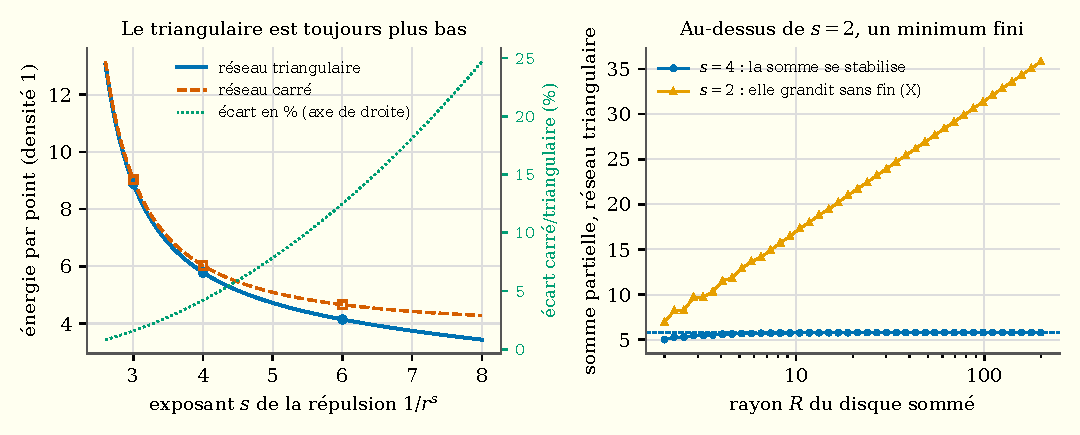
\includegraphics[width=\linewidth]{figures/c16_riesz}
\caption{À gauche~: énergie par point pour une répulsion $1/r^s$, réseau triangulaire contre réseau carré à densité~1,
recalculée ici (les marqueurs sont les valeurs publiées). À droite~: sommes partielles sur un disque de rayon~$R$,
qui se stabilisent pour $s=4$ et grandissent sans fin pour $s=2$.}
\label{fig:c16}
\end{figure}
